\begin{center}
	
	\Huge
	Előerősítő 70\,cm-es sávra
	
	\Large
	\url{https://github.com/simonyiszk/70cm_preamp}
	
	\Large
	HA5KFU projekt
	
	\Large
	Kiss Ádám (HA8KDA), Bazsó Márton (HA7BM), \\ Keresztes Botond, Agócs Dániel, Pápay Levente (HA3PL)
\end{center}

\tableofcontents

\listoffigures

\newpage

\section{Célkitűzés}
\label{sec:celkituzes}

Az erősítő hivatása, hogy a Schönherz kollégium tetejére telepített 70\,cm-es sávra készült antenna által fogott jeleket erősítse, közülük is elsősorban a SMOG-1 műholdét 437,345\,MHz-en.


\section{Kapcsolás}
\label{sec:kapcsolas}

Mivel az erősítő egy rádiófrekvencián elég \enquote{szennyezett} környékre kerül felszerelésre, így fontos egy jó szűrő alkalmazása ebben a fokozatban. Az akusztikus felületi hullámszűrők kitűnőek ilyen feladatokra, ugyanis nagyon meredek levágást biztosítanak a sávszéleken. Egy ilyen alkatrészt fellelni sem volt egyszerű, de beszerezni még bonyolultabbnak bizonyult, de végül a mouseren keresztül valahogyan sikerült. A választás az SF2446E\cite{SAW} néven futó áramkörre esett, melynek a minimum beszerzési mennyisége 10\,db volt.

Mint a legtöbb vételi berendezésben, itt is egy alacsony zajú előerősítő kerül a vételi lánc elejére. Előzőekben már épült egy hasonló kapcsolás egy ADL5523-as IC felhasználásával, de amikor kiderült, hogy az akusztikus szűrőből minimum 10-et kell rendelnünk, felmerült az ötlet, hogy gyártsunk le 10\,db áramkört, és a maradékra majd valahonnan kerítünk vevőt -- végül nem kellett sokat keresni, a nagy részük elkelt a klubon belül. Erősítőnek végül a Mini-Circuits PGA-103+\cite{PGA} terméke került kiválasztásra -- szintén a mouserről -- ugyanis kellően alacsony a zajtényezője, valamint 22\,dB erősítést ígér 400\,MHz-en, és végül, de nem utolsó sorban olcsóbb, mint egy ADL5523-as.

\begin{figure}[!ht]
	\centering
	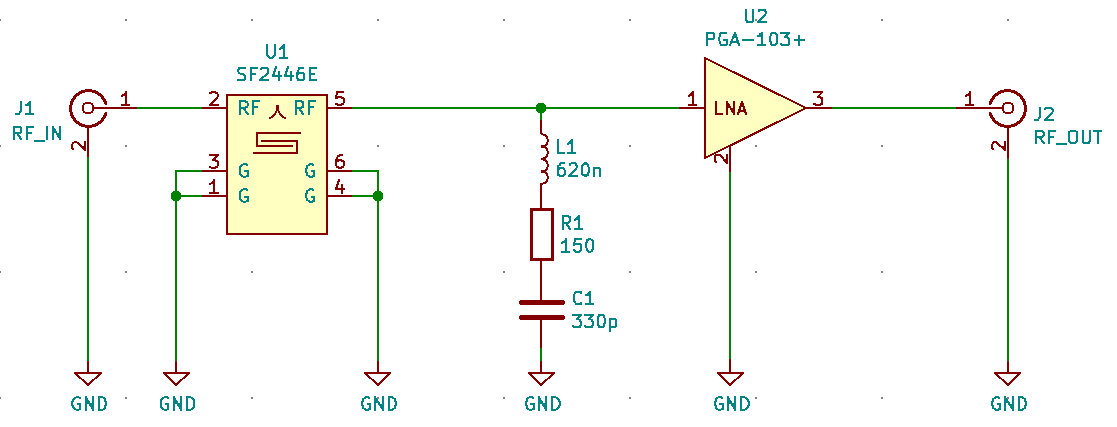
\includegraphics[keepaspectratio, width=0.8\textwidth]{kapcsolas.png}
	\caption{Az előerősítő kapcsolása}
	\label{fig:LNA_sch}
\end{figure}

Alapesetben az erősítő a szűrő elé kerülne, ugyanis az eredő rendszernek így kedvezőbb lesz a jel-zaj viszonya. Viszont mint említésre került, a telepítési hely RF szempontból elég \enquote{szennyezett}, így félő, hogy a nagy sávszélességű erősítőnket könnyen túlvezérlik a számunkra érdektelen jelek. Ebből a meggondolásból a szűrőt az erősítő elé helyeztük, hogy csökkentsük a bele jutó összteljesítményt.

Amikor a NYÁK már majdnem gyártásba lett adva, Levente felhívta a figyelmünket egy kiegészítő dokumentumra\cite{PGA_comp}, mely az erősítőhöz megad egy kompenzáló hálózatot, ugyanis nélküle az áramkör 100\,MHz alatt nem lenne stabil. Így ez a 3 passzív alkatrészből álló kiegészítés az utolsó pillanatban még a tervre került. A végleges kapcsolás az \ref{fig:LNA_sch}-es ábrán látható.


\section{NYÁK}
\label{sec:nyak}

A hordozót elég kis méretűre meg lehetett csinálni, ugyanis mindösszesen 7 alkatrészt tartalmaz. A jelet vivő tápvonal úgy lett kialakítva, hogy a hullámimpedanciája 50\,$\Omega$-os legyen, ez főként azért lett ilyenre megcsinálva, hogy Marci gyakorolja CST-s szimulációs képességeit. Az elkészült rajzolat a \ref{fig:nyak}-es ábrán látható, mely egy kétrétegű, 1\,mm vastag hordozóra lett elkészítve.

\begin{figure}[!ht]
	\centering
	\begin{subfigure}[b]{0.49\textwidth}
		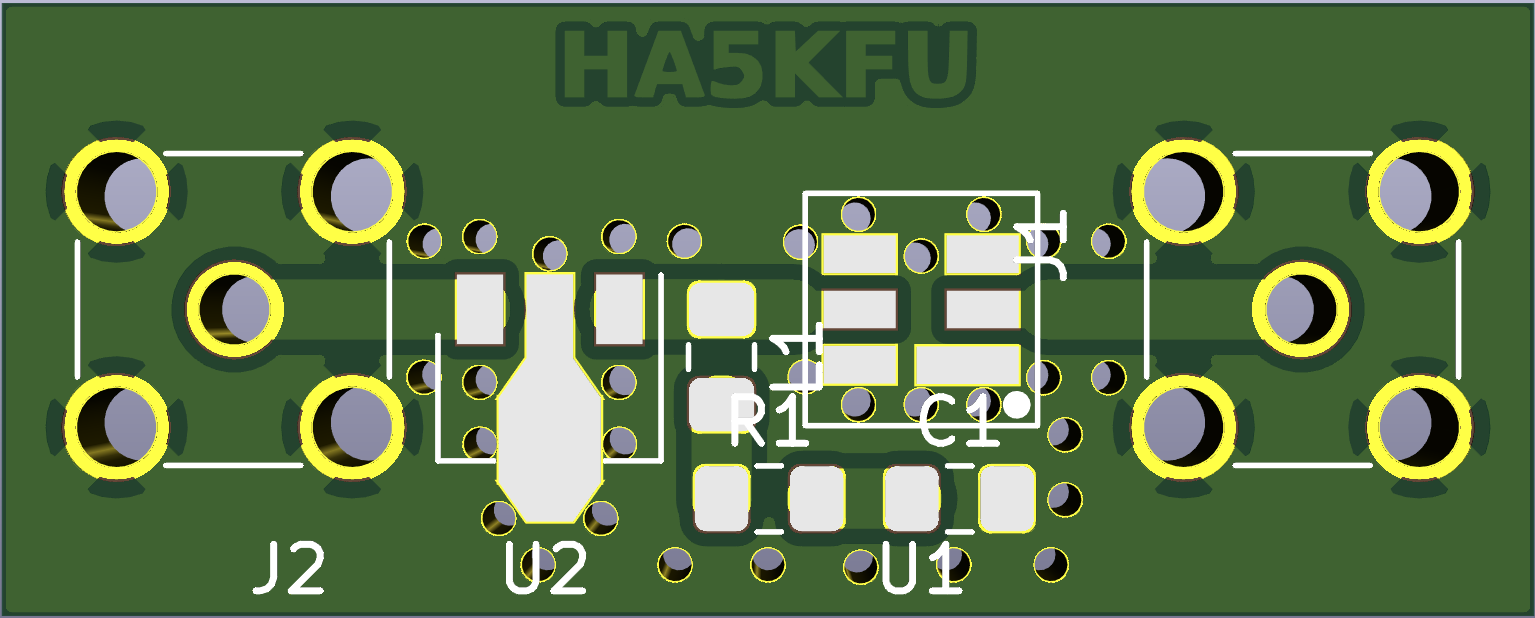
\includegraphics[keepaspectratio, width=\textwidth]{nyak_eleje.png}
		\caption{NYÁK eleje}
		\label{fig:nyak_elol}
	\end{subfigure}
	\begin{subfigure}[b]{0.49\textwidth}
		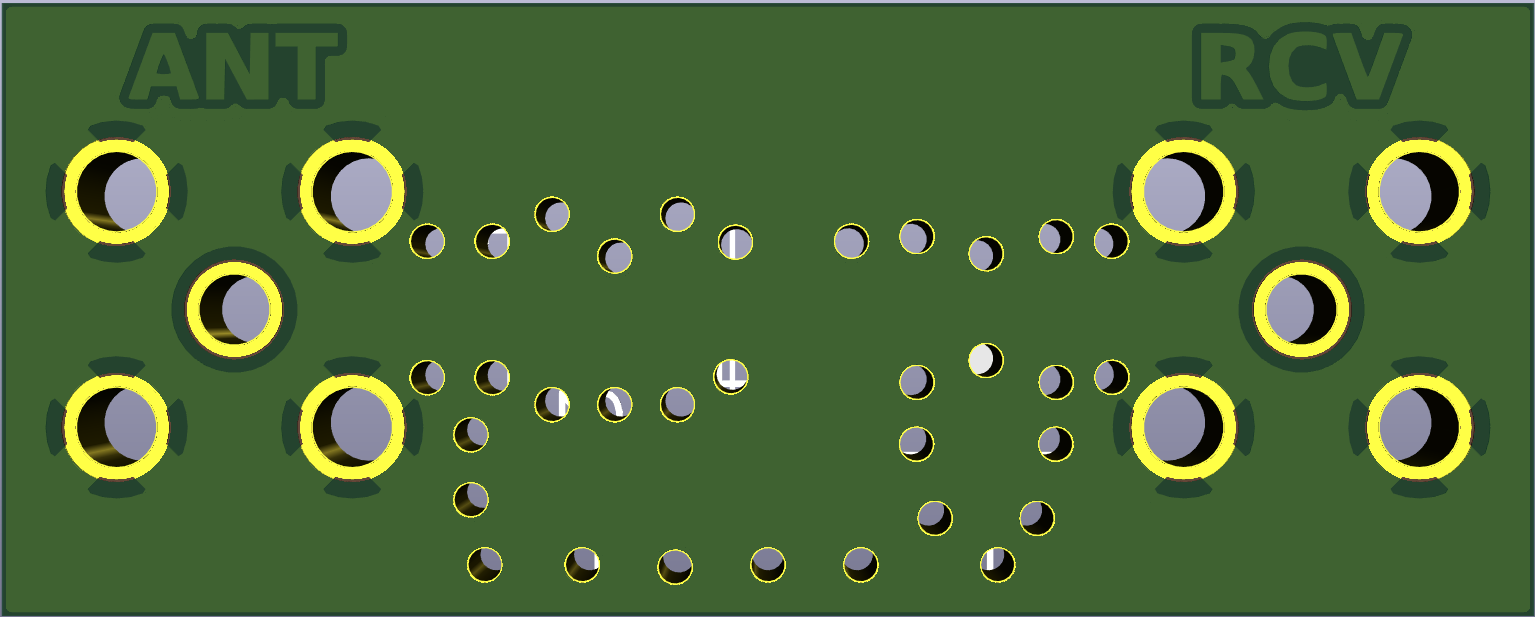
\includegraphics[keepaspectratio, width=\textwidth]{nyak_hatulja.png}
		\caption{NYÁK hátulja}
		\label{fig:nyak_hatul}
	\end{subfigure}
	\caption{NYÁK terv a KiCAD 3D nézetében}
	\label{fig:nyak}
\end{figure}

Némi megfontolást igényelt, hogy az áramkörünk hordozóját az Elektronikai Technológia Tanszéken, vagy egy keleti üzemben gyártassuk le. A döntő szempont végül a sebesség volt, ugyanis a SMOG-1 indítása rohamosan közeledett, és szerettünk volna elkészülni vele, így az ETT-re esett a választás, ugyanis a keletről történő postázás időtartama viszonylag hosszú és olykor kiszámíthatatlan.


\section{Mérés 1}
\label{sec:meres1}

Miután elkészült néhány példány az áramkörből, ezek bemérésre kerültek a BME V1 épületében található Rohde \& Schwarz laboratóriumban. A méréshez használt eszközök egy R\&S ZVRE vektor hálózat analizátor, illetve egy R\&S ESCS30 típusú jelanalizátor, mellyel gerjedést mértünk a 100\,kHz - 1\,GHz tartományon -- utóbbi mérési eredmények külön nem kerültek elmentésre. Az áramkörök táplálásához Yume tápfeladóját, egy LM7805-öst, és egy R\&S NGMO2-es típusú labortápot használtunk, melynek kimenetét 8\,V-ra állítottuk.

A bemért áramkörök:

\begin{itemize}
	\item \#1: Szűrő + erősítő + kompenzáló hálózat
	\item \#2: Szűrő + erősítő + kompenzáló hálózat
	\item \#2.5: \#2-es áramkör javítás után (erősítő nem megfelelő forrasztása)
	\item \#3: Szűrő + erősítő
\end{itemize}

\newpage

Mivel a klubban nem voltak fellelhetők a kompenzáló hálózathoz szükséges pontos értékek, így az a következő értékekkel lett megvalósítva:

\begin{itemize}
	\item L1 220\,nH
	\item R1 150\,$\Omega$
	\item C1 330\,pF
\end{itemize}

Az áramkörökről összesen 14 mérés készült (ebből 13-at el is mentettünk, az utolsót elfelejtettük). A következőkben a legfontosabbak kerülnek ismertetésre, a többit pedig a Függelék (\ref{sec:fuggelek}) tartalmazza.

\subsection{\#1-es áramkör}
\label{subsec:1es_aramkor}

A \ref{fig:erosito1}-as ábrán az áramkör átvitele ($S_{21}$ paraméter) látható.

\begin{figure}[!ht]
	\centering
	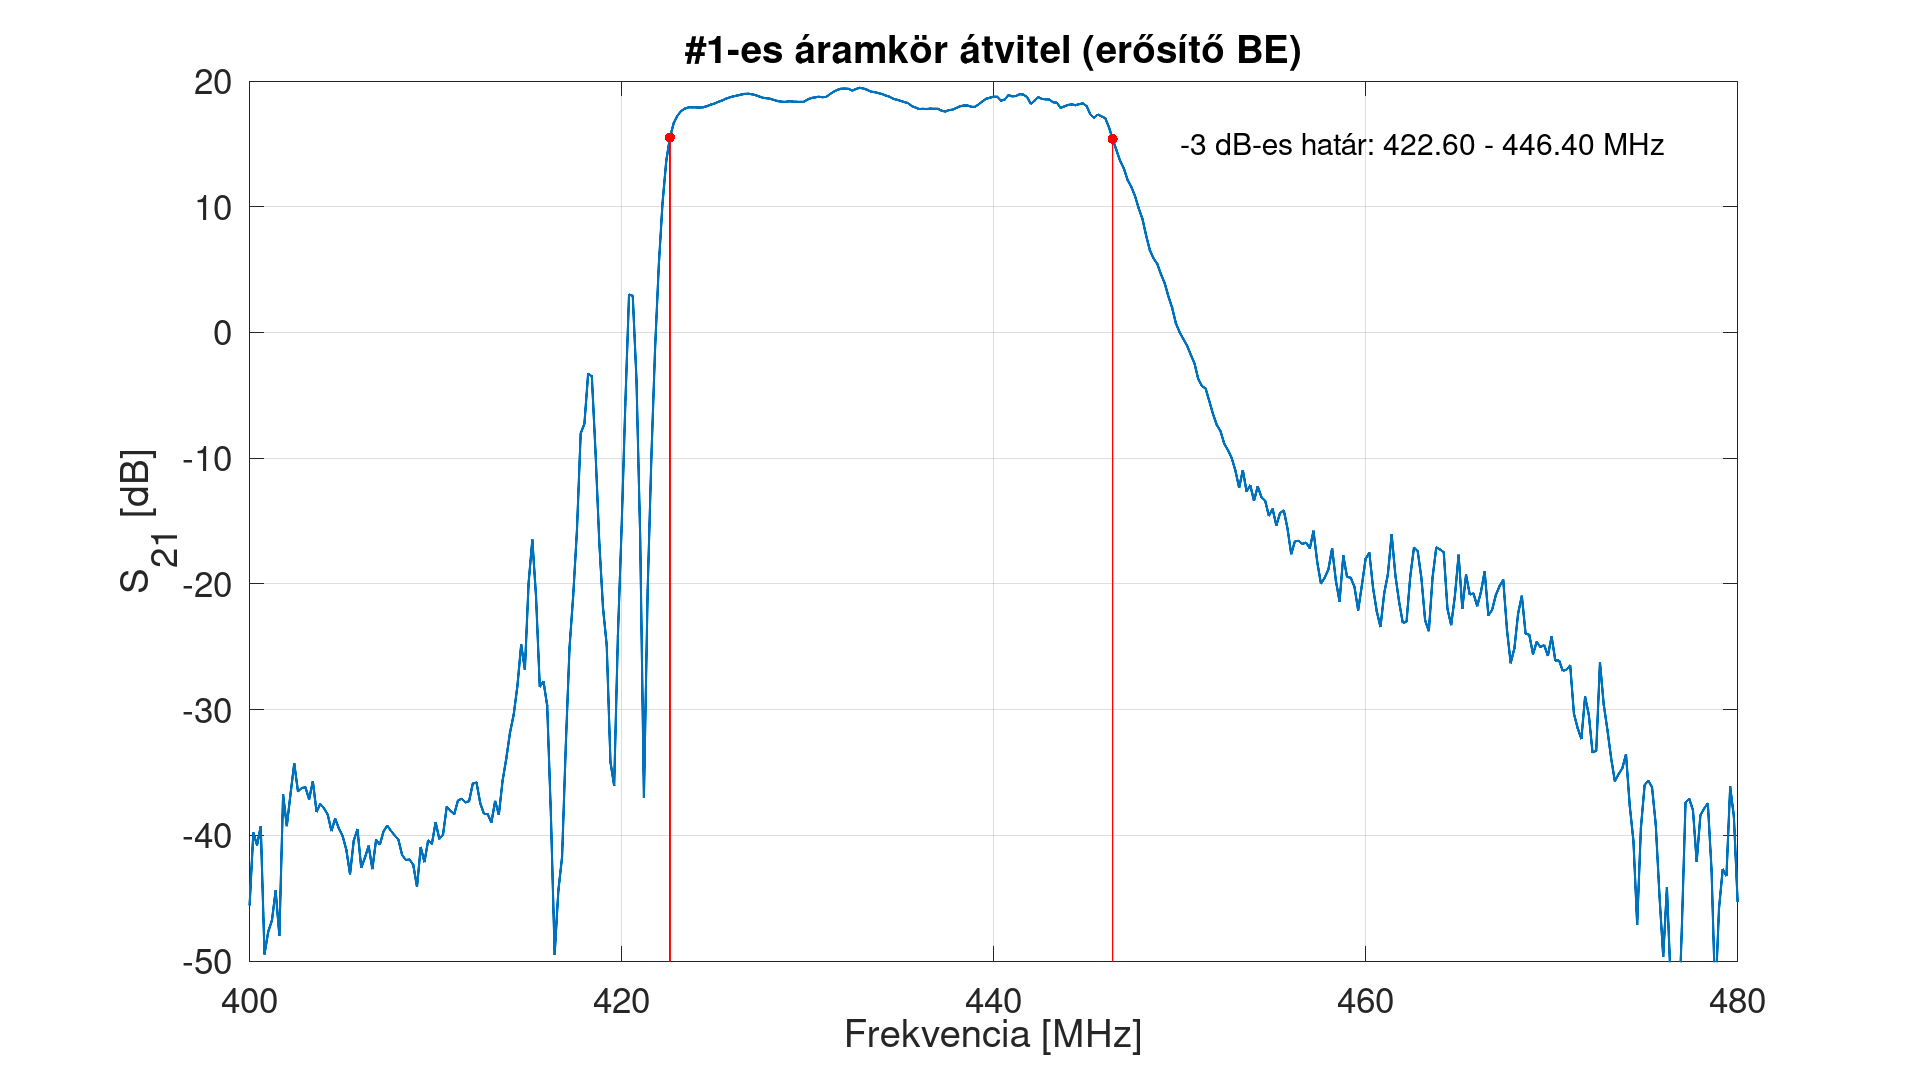
\includegraphics[keepaspectratio, width=\textwidth]{aramkor1_4.png}
	\caption{\#1-es erősítő átvitele}
	\label{fig:erosito1}
\end{figure}

A mérés nagyságrendileg megegyezik az elvárásokkal. Az erősítőtől ebben a tartományban 22\,dB erősítést várunk, míg a szűrő nagyjából 2\,dB-t csillapít, avagy közel a várt eredményt kaptuk. A sávszélesség is jól egyezik a szűrő adatlapjában\cite{SAW} megadott 23\,MHz-el. Az erősítő áramfelvétele is (95\,mA) közel van az adatlapi\cite{PGA} értékhez, így összességében kijelenthető, hogy az áramkör az elvártnak megfelelően működik.

A vizsgálatok során nem találtunk gerjedésre utaló jeleket, így kijelenthető az is, hogy az alternatív értékekből összerakott kompenzáló hálózat is megfelelően ellátja feladatát.


%\newpage

\subsection{\#2-es áramkör}
\label{subsec:2es_aramkor}

Ez az áramkör először nem működött rendeltetésszerűen, ugyanis az erősítése gyanúsan alacsony volt. Egy gyors mikroszkóp alatti szemrevételezés után kiderült, hogy ennek oka, a nem megfelelően beforrasztott erősítő volt. A hiba javítása után a \ref{fig:erosito2}-es ábrán látható átvitelt kaptuk.

\begin{figure}[!ht]
	\centering
	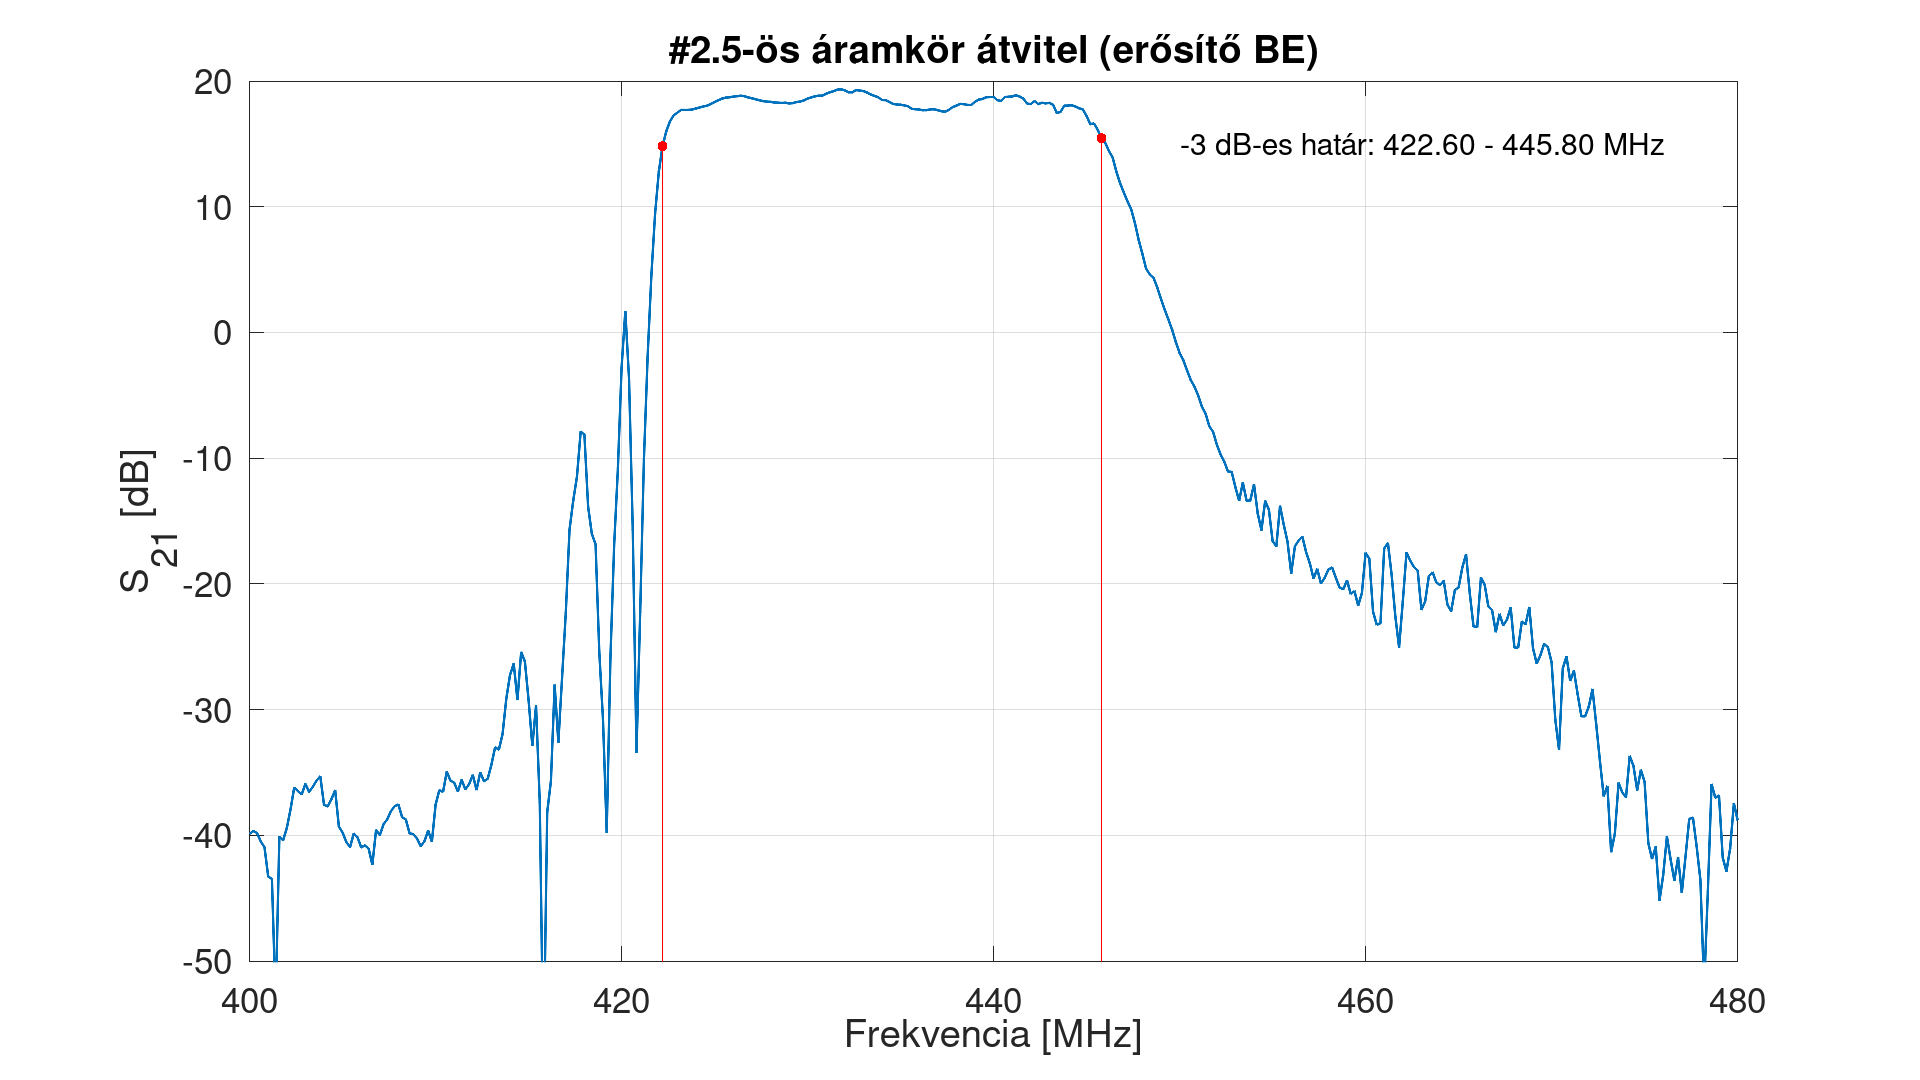
\includegraphics[keepaspectratio, width=\textwidth]{aramkor2_14.png}
	\caption{\#2.5-ös erősítő átvitele}
	\label{fig:erosito2}
\end{figure}

Látható, hogy az átvitel jellege megegyezik az \#1-es áramkörnél mérttel, így erről is elmondható, hogy megfelelően működik. Ez a kapcsolás eleinte mutatott gerjedés gyanús jeleket, melyeket a későbbiek során nem sikerült reprodukálnunk. Feltételezhetően a spektrumbeli kitüremkedések egy tranziensjelenség miatt következtek be. A további mérések során az áramkör stabilnak bizonyult.


\subsection{\#3-as áramkör}
\label{3as_aramkor}

Miután megtaláltuk a kiegészítőt az adatlaphoz\cite{PGA_comp}, kíváncsiak voltunk, hogy vajon hogyan viselkedne az áramkör, ha nem építjük bele az ajánlott kompenzáló hálózatot. Ezért a harmadik áramkör csak a szűrőt és az erősítőt tartalmazta. A mérés eredménye a \ref{fig:erosito3}-ös ábrán látható.

\begin{figure}[!ht]
	\centering
	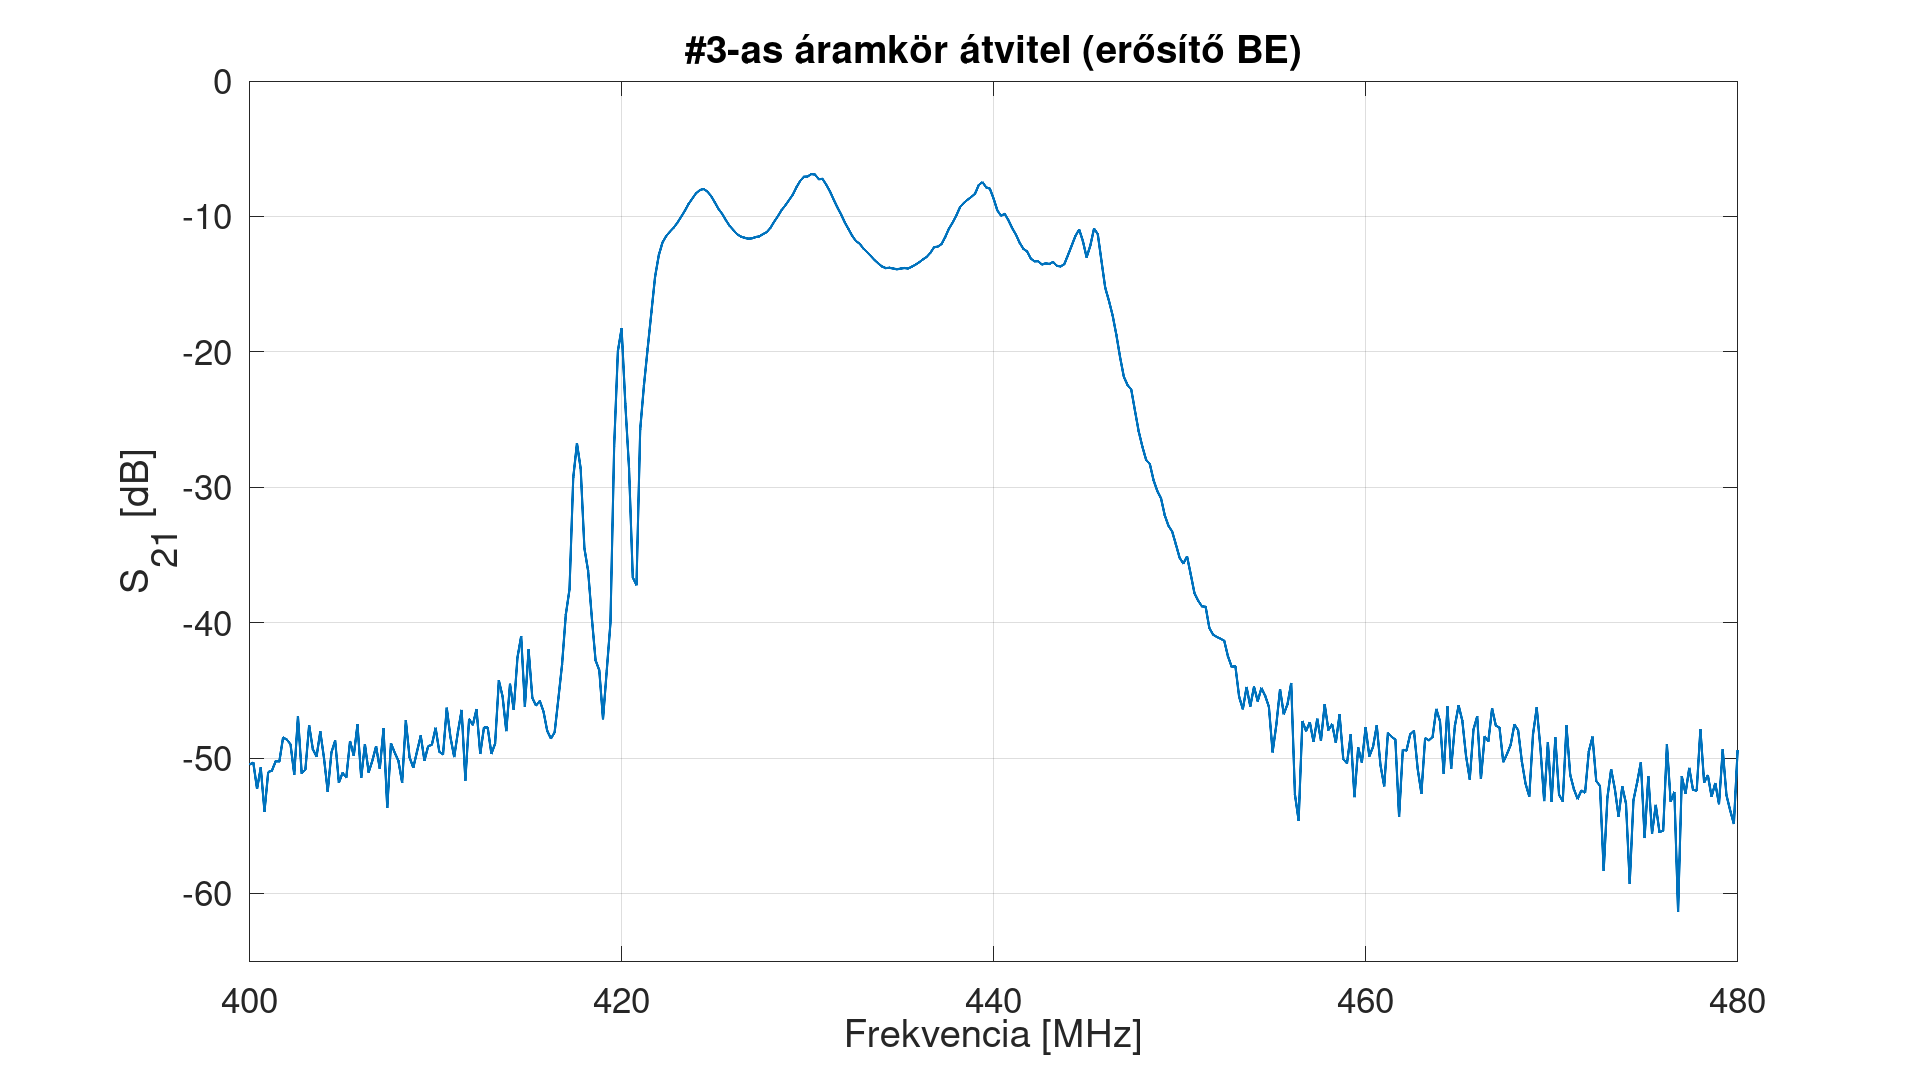
\includegraphics[keepaspectratio, width=\textwidth]{aramkor3_12.png}
	\caption{\#3-as erősítő átvitele}
	\label{fig:erosito3}
\end{figure}

Megfigyelhető, hogy a szűrő amplitúdómenete az áteresztő sávban jóval hullámosabb az adatlapban\,\cite{SAW} és az előző mérésekben látottnál. Ez a szűrő illesztetlenségére utalhat, ami azért különös, mert elméletileg minden eszközünk ki- és bemeneti impedanciája is 50\,$\Omega$-os. Látható az is, hogy az erősítő bekapcsolásakor is csak -10\,dB az átvitel, ami nem éppen nevezhető erősítőnek. Ezt a kapcsolást is megvizsgáltuk gerjedés szempontjából, de itt sem tapasztaltunk semmi ráutaló jelet.

1-2 nappal a mérések után felmerült bennem, hogy lehet, ennél a kapcsolásnál is volt nem megfelelő forrasztás, ugyanis szerintem a kompenzáló hálózat hiányának nem szabadna ekkora csillapítást okoznia (30\,dB-lel voltunk az elvárt szint alatt). A szűrőnek a megváltozott amplitúdómenetéből valószínűsíthető, hogy összességében a kompenzálóhálózat hiánya befolyással van az áramkör viselkedésére, viszont nem zárható ki, hogy volt egyéb tényező -- a kiegészítő hálózaton kívül -- ami befolyásolta az eredményt. Ezért nem jelenthető ki egyértelműen, hogy ez a mérés a kompenzáló hálózat átvitelre gyakorolt hatását szemlélteti.


\section{Mérés 2}
\label{sec:meres2}

Miután az első mérésekkel igazoltuk, hogy az alapkoncepció működőképes, megrendeltük a szükséges passzív alkatrészeket és csatlakozókat\cite{90es_SMA}, majd ismét beköltöztünk egy délután erejéig a BME V1 épületében található Rohde \& Schwarz laboratóriumba, hogy beforrasszuk az áramköröket, és méréssel igazoljuk működésüket.

A méréshez használt eszközök egy R\&S ZVRE vektor hálózat analizátor, illetve egy R\&S ESCS30 típusú jelanalizátor, mellyel gerjedést mértünk a 100\,kHz - 1\,GHz tartományon -- utóbbi mérési eredmények külön nem kerültek elmentésre. Az áramkörök táplálásához Yume tápfeladóját, egy LM7805-öst, és egy R\&S NGMO2-es típusú labortápot használtunk, melynek kimenetét 8\,V-ra állítottuk. A mérési elrendezés a \ref{fig:elrendezes}-es ábrán látható -- a labortápot leszámítva.

\begin{figure}[!ht]
	\centering
	\begin{minipage}[b]{0.49\textwidth}
		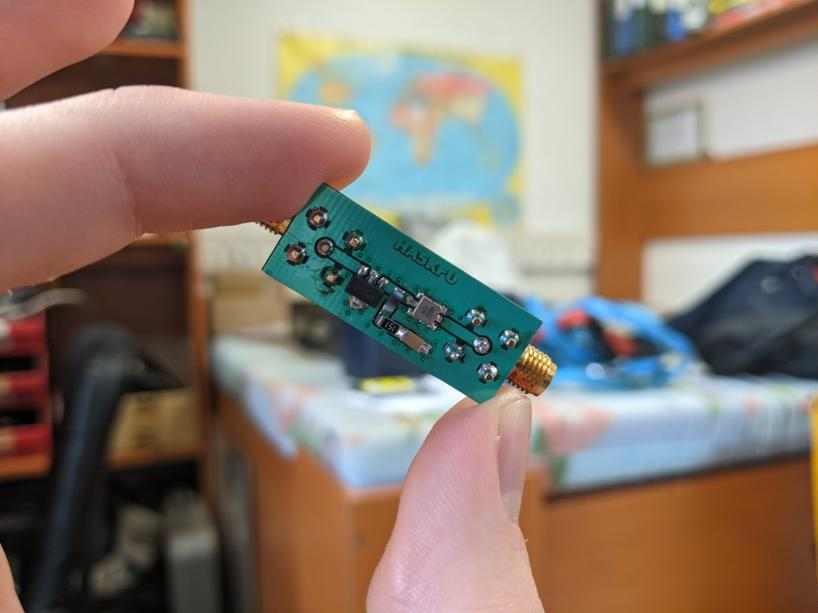
\includegraphics[width=\textwidth, keepaspectratio]{beforrasztott.jpg}
		\caption{Egy beforrasztott áramkör}
		\label{fig:beforrasztott}
	\end{minipage}
	\begin{minipage}[b]{0.49\textwidth}
		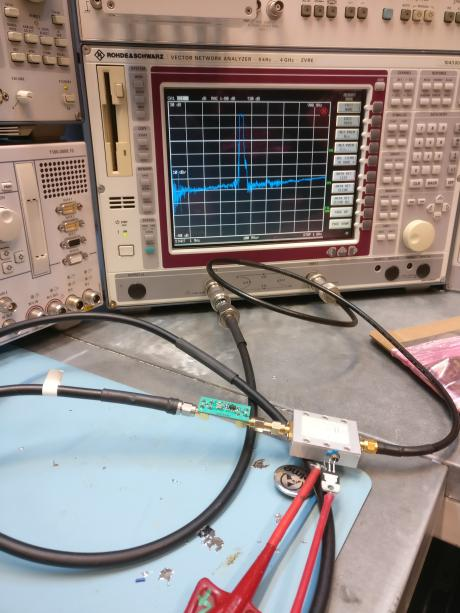
\includegraphics[width=\textwidth, keepaspectratio]{elrendezes.jpg}
		\caption{Mérési elrendezés}
		\label{fig:elrendezes}
	\end{minipage}
\end{figure}

A módszertanon annyit változtattunk az előző alkalomhoz képest, hogy a VNA-t úgy kalibráltuk, hogy a két portját összecsatoltuk, közbeiktatva a tápfeladót, és rákapcsolva a tápegységet. Így -- mint látni fogjuk -- a várthoz közelebbi eredményeket kaptunk, mint előző alkalommal, amikor csak a mérőkábelek lettek kikompenzálva.

Mivel a Lomex-ben nem voltak kaphatók pont azok az értékek, melyeket az előzőekben kipróbáltunk, így a kompenzáló hálózat értékei a következők lettek:

\begin{itemize}
	\item L1 330\,nH\cite{L1}
	\item R1 150\,$\Omega$\cite{R1}
	\item C1 330\,pF\cite{C1}
\end{itemize}

Az alábbi áramkörök kerültek megépítésre és bemérésre (az összes alkatrészt tartalmazzák, kivétel ahol másként van feltüntetve):

\begin{itemize}
\item \#0: \#7-es áramkör kompenzálóhálózat nélkül
\item \#2.5: lásd: \ref{sec:meres1} és \ref{subsec:2es_aramkor} pont
\item \#3.5: \#3-as áramkör javítás után (szűrő nem megfelelő forrasztása)
\item \#4
\item \#5
\item \#6
\item \#7
\item \#8
\end{itemize}

A nap végére az összes beforrasztott áramkör működőképes volt, és az elvártnak megfelelően üzemelt.

Mivel kiderült, hogy az előző alkalommal valóban egy rosszul beforrasztott áramkörön tanulmányoztuk a kompenzáló hálózat hatását, így megismételtük a mérést, ezúttal különös tekintettel a forrasztásra. A mérési eredményeket a \ref{fig:kompenzalo_halozat}-as ábra veti össze.

\begin{figure}[!ht]
	\centering
	\begin{subfigure}[b]{\textwidth}
		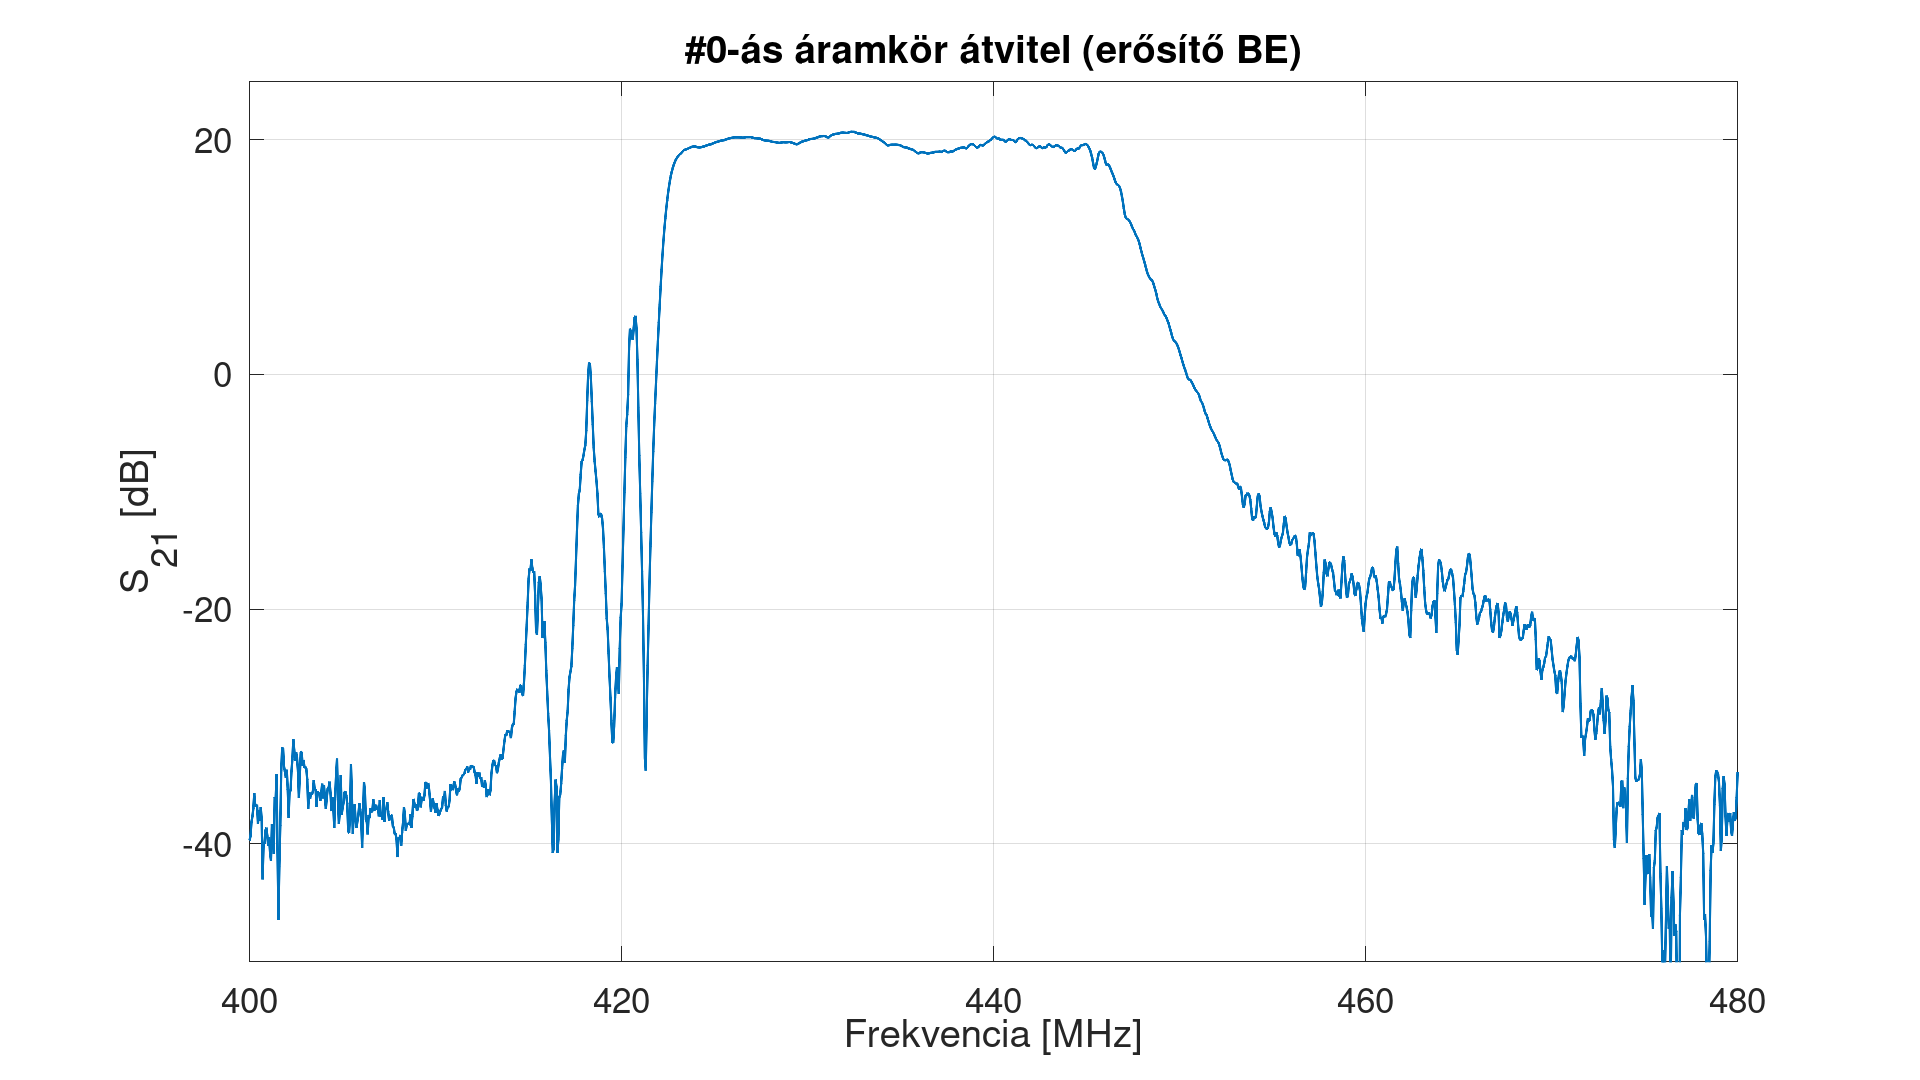
\includegraphics[keepaspectratio, width=\textwidth]{aramkor0_02.png}
		\caption{Kompenzáló hálózat nélkül}
		\label{fig:erosito0}
	\end{subfigure}
	\begin{subfigure}[b]{\textwidth}
		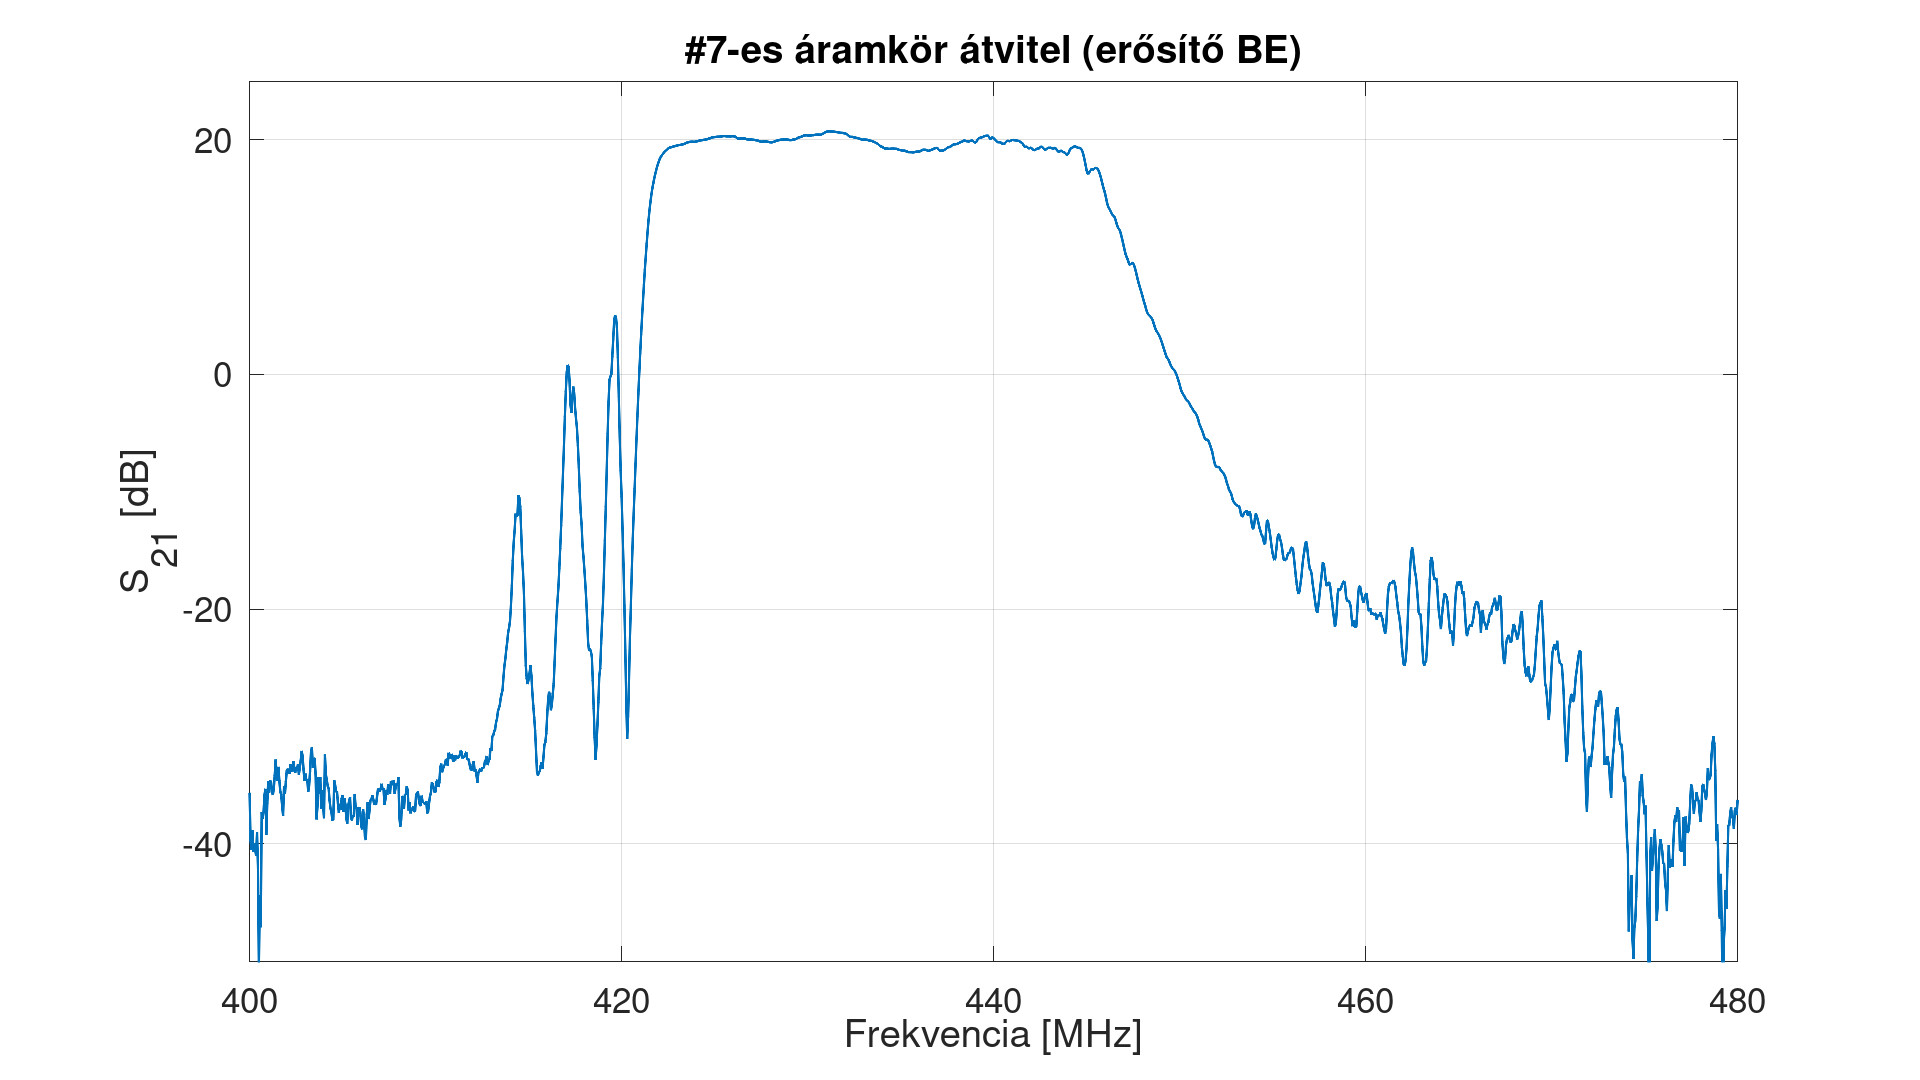
\includegraphics[keepaspectratio, width=\textwidth]{aramkor7_72.png}
		\caption{Kompenzáló hálózattal}
		\label{fig:erosito7}
	\end{subfigure}
	\caption{Kompenzálás hatásának vizsgálata}
	\label{fig:kompenzalo_halozat}
\end{figure}

Látható, hogy a két áramkör között nincsen jelentős eltérés az átviteli sávban, mindössze annyi különbség figyelhető meg, hogy a \ref{fig:erosito0} esetben az áteresztő sáv enyhén felfelé tolódott el frekvenciatartományban. A jelanalizátoron végzett mérés sem mutatott észlelhető gerjedést a 100\,kHz - 1\,GHz-es tartományban.

Végeredményben a mi méréseink alapján ezen alkalmazáshoz nem nélkülözhetetlen a kompenzáló hálózat, ennek ellenére az ajánlásnak megfelelően beforrasztottuk őket.


\subsection{Árnyékolás}
\label{subsec:arnyekolas}

Mivel a HA5KFU-nak gyártott példány egy erősen \enquote{RF szennyezett} környezetbe kerül -- Schönherz teteje -- így úgy döntöttünk, hogy a tetőre kerülő példányt (\#3.5-ös áramkör) bedobozoljuk, hogy védjük ezen zavarok ellen. Az árnyékoló dobozba\cite{doboz} szerelt áramkör a \ref{fig:arnyekolas}-es ábrán látható (az egyes csatlakozók funkcióját természetesen feliratozással jeleztük a szintén az ábrán látható alkoholos filctollal). Az egyszerűbb dobozolás érdekében itt a korábban látott $90^{\circ}$-os SMA csatlakozók helyett egyeneseket használtunk\cite{egyenes_SMA}.

\begin{figure}[!ht]
	\centering
	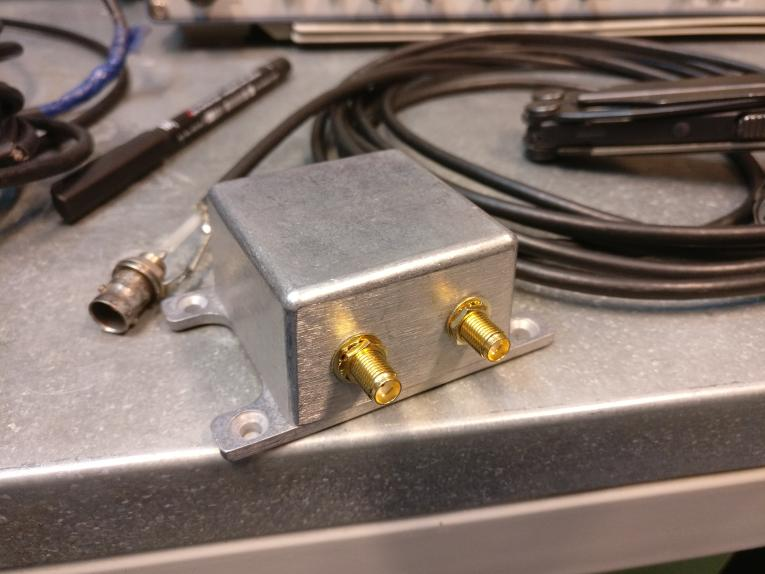
\includegraphics[keepaspectratio, width=0.8\textwidth]{arnyekolo_doboz.jpg}
	\caption{Az árnyékolt erősítő}
	\label{fig:arnyekolas}
\end{figure}

A jelanalizátorral végzett mérések a következő eredményt adták:

Árnyékolás nélkül a spektrumban kb. -80\,dBm szintű csúcsok láthatóak 100\,MHz, 800\,MHz és 900\,MHz környékén, melyek rendre az FM adók, LTE hálózat illetve a GSM hálózat. Az árnyékolt áramkör összeszedett zavarait nem tudtuk kimutatni, ugyanis nem türemkedtek az analizátor -90\,dBm-es zajszintje fölé.

A mérés alapján kijelenthető, hogy az árnyékolás kedvező hatással van a zajszintre, az összeszedett zavarok szintjét -90\,dBm alá csökkentette (a mérés helyszínén).


\subsection{Nem párhuzamos diódapár}
\label{subsec:diodak}

Tartunk tőle, hogy a tetőre kihelyezett gamma illesztésű antenna elektrosztatikusan feltöltődik, és egy esetleges kisülés károsítja a felületi szűrőnket. Ennek orvoslására egy ellentétes polaritással bekötött diódapárt helyeztünk a szűrő elé (a \ref{fig:diodak}-es ábrának megfelelően), hogy az esetlegesen felgyülemlő töltéseket ki tudja egyenlíteni. A választásnál fontos volt, hogy kis kapacitású diódákat\cite{dioda} használjunk, mivel ezek esetlegesen elhangolhatnák a szűrőt, és az átviteli sávot.

\begin{figure}[!ht]
	\centering
	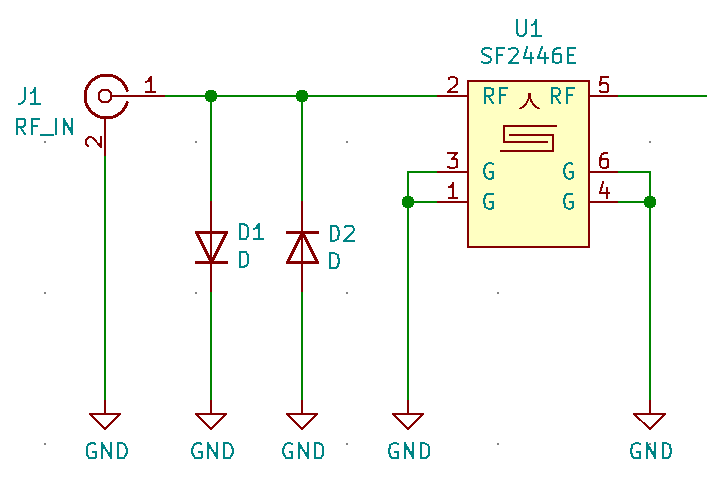
\includegraphics[keepaspectratio, width=0.8\textwidth]{diodak.png}
	\caption{Nem párhuzamos diódapár}
	\label{fig:diodak}
\end{figure}

Mivel ez egy utólagos ötlet volt, így ezen alkatrészeknek nem lett külön hely kialakítva a NYÁK-on, hanem a csatlakozó lábai közé lettek \enquote{begányolva}.

A beépítés utáni mérések azt mutatták, hogy a beiktatott diódák nem befolyásolják kimutatható mértékben az erősítő átvitelét.